\documentclass[a4paper,12pt,titlepage]{article}
\usepackage[utf8]{inputenc}
\usepackage{graphicx} % Required for inserting images
\usepackage[spanish,es-tabla]{babel}
\usepackage[none]{hyphenat}
\usepackage[justification=centering]{caption}
\usepackage{subcaption}
\usepackage{amssymb, amsmath}
\usepackage{gensymb}
\usepackage{fancyhdr}
\usepackage{wrapfig}


\lhead{Momento de inercia}
\rhead{Gonzalo Bastos González}

\pagestyle{fancy}

\title{Momento de inercia}
\author{Gonzalo Bastos González}

\begin{document}

\maketitle
\tableofcontents

\newpage

\section{Objetivos e introducción teórica}

Esta práctica gira alrededor del concepto de momento de inercia y tiene dos objetivos principales:

\begin{itemize}
    \item Medir experimentalmente el momento de inercia de diferentes cuerpos
    \item Verificar el teorema de Steiner
\end{itemize}

Para comenzar con nuestra práctica en primer necesitamos unas bases teóricas sobre las que realizar nuestros experimentos. La práctica parte del concepto de momento de inercia, magnitud que se define como la cuantificación de la inercia de rotación de un cuerpo. Matemáticamente el concepto de momento de inercia de un sistema de partículas se define como:

\begin{equation}
    I = \sum_i^N m_i r_i^2
\end{equation}

Esta fórmula puede generalizara para cuerpos de masa continua, que son con los que trabajamos, con la siguiente expresión:

\begin{equation}
    I = \int r^2 dm
    \label{Def MI}
\end{equation}

Si aplicamos esta expresión a determinados cuerpos geómetricos simples podemos obtener una expresión simplificada para su momento de inercia respecto a su eje de simetría:

\begin{equation}
    \begin{gathered}
        \text{Disco: } I=\frac{MR^2}{2} \\
        \text{Cilindro: } I = \frac{MR^2}{2}\\
        \text{Esfera: } I = \frac{2MR^2}{5} \\
        \text{Barra: } I = \frac{ML^2}{12}
        \label{MI cuerpos geometricos}
    \end{gathered}
\end{equation}

Siendo $M$ la masa del cuerpo, $R$ su radio y $L$ su longitud.
\par A partir de la definición de momento de inercia podemos intuir que esta magnitud va a presentar una gran relación con la rotación de los cuerpos y, por tanto, las magnitudes que la definen. Partiremos de la ecuación fundamental del movimiento de rotación:

\begin{equation}
    \vec{M} = \frac{d\vec{L}}{dt}
\end{equation}

Donde se relaciona el momento de la fuerza que produce la rotación ($\vec{M}=\vec{R}\times \vec{F}$) con la derivada del momento angular $\vec{L}$. En un sólido rígido el momento angular se puede expresar como:

\begin{equation}
    \vec{L} = I \vec{\omega}
\end{equation}

Siendo $\vec{\omega}$ la velocidad angular. Cuando el giro se produce sobre uno de los ejes principales del cuerpo el momento angular tiene la misma dirección que $\vec{\omega}$ y podemos emplear la expresión anterior en módulos ($L=I_e\omega$).

\par Para nuestra práctica mediremos el momento de inercia respecto a un eje a partir del período de oscilación de su rotación cuando se le hace girar sometido a la fuerza recuperadora de un resorte elástico. El momento de esa fuerza recuperadora cumple la siguiente relación:

\begin{equation}
    M = -D\varphi
    \label{Constante resorte}
\end{equation}

Donde $D$ es una constante propia del resorte y $\varphi$ es el ángulo girado. A partir de esta ecuación vamos a buscar una relación que nos permita calcular el momento de inercia del cuerpo respecto al eje a partir del momento de la fuerza, que podremos determinar experimentalmente:

\begin{equation}
    M = \frac{dL}{dt};\; L=I\omega;\; \omega = \frac{d\varphi}{dt} \Rightarrow M = I \frac{d^2\varphi}{dt^2}
\end{equation}

Teniendo en cuenta la expresión anterior y la Ec.\ref{Constante resorte} obtenemos la siguiente expresión:

\begin{equation}
    \frac{d^2\varphi}{dt^2} = -\frac{D}{I}\varphi
\end{equation}

Esta es la ecuación diferencial que describe el comportamiento de un oscilador simple, si la resolvemos obtenemos la siguiente expresión que nos ayuda a modelizar la oscilación:

\begin{equation}
    \varphi(t) = \varphi_0 \cos\left (\sqrt{\frac{D}{I}}t+\phi_0\right ) 
\end{equation}

El período de este movimiento armónico viene dado por la siguiente expresión:

\begin{equation}
    T = 2\pi\sqrt{\frac{I}{D}}
    \label{Periodo oscilacion}
\end{equation}


Esta expresión nos permitirá calcular el momento de inercia de nuestro cuerpo midiendo su período de oscilación cuando se somete a la fuerza recuperadora del resorte, algo mucho más fácil de medir experimentalmente. Esta igualdad nos servirá como fundamento para calcular todos los momentos de inercia medidos a lo largo de toda la práctica.

\par La segunda parte de la práctica se centra en verificar el teorema de Steiner, que afirma que el momento de inercia de un sólido rígido respecto a un eje es igual al momento de inercia respecto a otro eje paralelo que pasa por el centro de masas, más el producto de la masa del sólido por la distancia que separa ambos ejes al cuadrado. Matemáticamente se puede expresar como:

\begin{equation}
    I_{ee} = I_0 + md^2
\end{equation}

\section{Materiales y metodología}

Los materiales empleados para el estudio de sus propiedades fueron:

\begin{itemize}
    \item Disco perforado, de $381,39 \;g$ de masa y $29,9 \; cm$ de diámetro.
    \item Esfera maciza, de $659,23 \; g$ de masa y $13,8 \; cm$ de diámetro
    \item Cilindro macizo, de $384,29 \; cm $ de masa y $10 \; cm$ de diámetro
    \item Barra rígida, de $65,7 \; cm$ de longitud
\end{itemize}
La incertidumbre de las medidas masas viene dada por la precisión instrumental de la balanza:
\begin{equation}
    s(m) = 0,01 \; g
\end{equation}
Por otro lado, la incertidumbre de las medidas realizadas con la regla de los diámetros y la longitud de la barra viene dada por la precisión instrumental de la regla empleada:
\begin{equation}
    s(x) = 0,001 \;m
\end{equation}
Para realizar las medidas contamos con los siguientes instrumentos:

\begin{itemize}
    \item Balanza
    \item Recta milimetrada
    \item Soporte giratorio dotado de un resorte
    \item Detector fotoeléctrico empleado para medir semiperíodos
    \item Dinamómetro
\end{itemize}

En la siguiente figura podemos ver los materiales empleados:

\begin{figure}[h!]
    \centering
    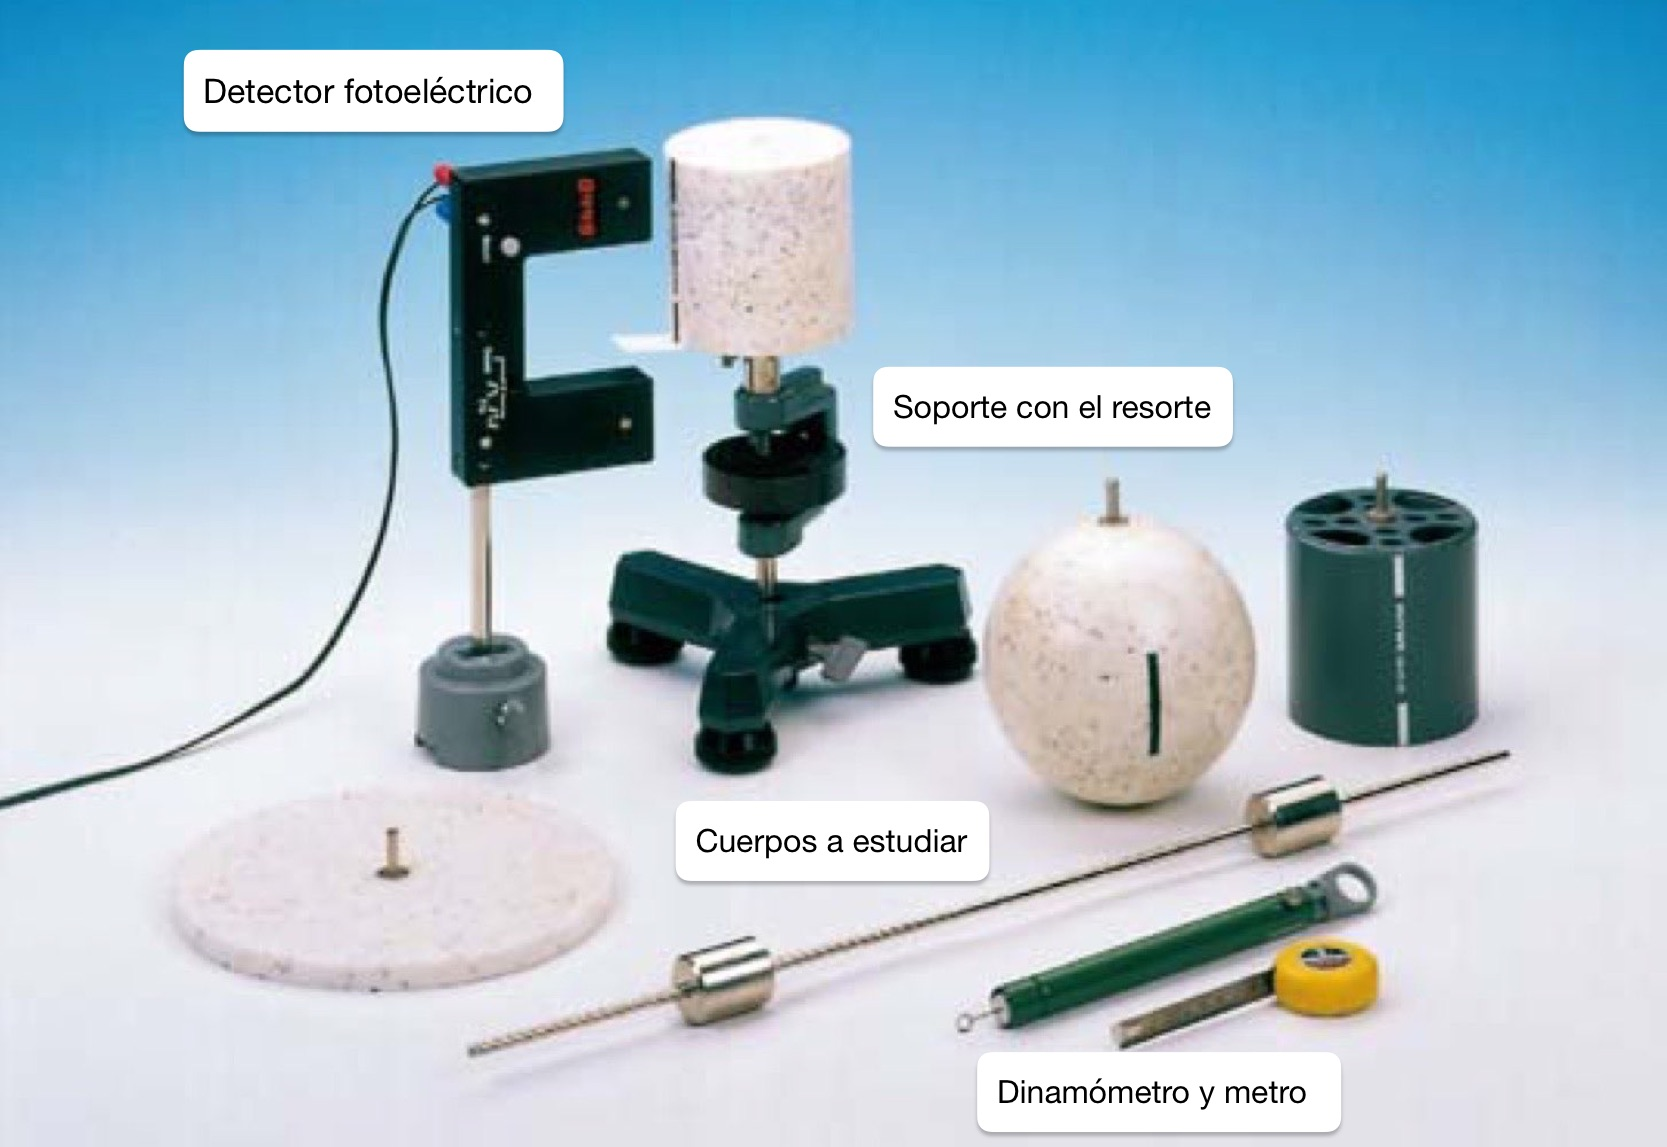
\includegraphics[width=0.75\linewidth]{Images/Material MI-1.jpg}
    \caption{Materiales empleados}
\end{figure}

El procedimiento experimental seguido en cada una de las dos partes de la práctica se detallará a continuación:

\subsection{Determinación del momento de inercia de diferentes cuerpos}

Esta primera parte de la práctica se centra en determinar los momentos de inercia de diferentes cuerpos respecto a su eje de simetría. Para ello aplicaremos la Ec.\ref{Periodo oscilacion}, que relaciona el momento de inercia del cuerpo con su período de oscilación. No obstante, por comodidad a la hora de trabajar con el detector fotoeléctrico hemos decidido trabajar con semiperíodos. Por tanto la expresión de la Ec.\ref{Periodo oscilacion} se transforma en:

\begin{equation}
    T_{1/2} = \pi \sqrt{\frac{I}{D}}
    \label{SemiT osc}
\end{equation}

Como observamos en la expresión anterior la relación entre el semiperíodo y el momento de inercia depende también de la constante $D$ del resorte, \textit{a priori} desconocida. Para calcular el valor de esa constante partiremos de la Ec.\ref{Constante resorte} ($M=-D\varphi$R) y realizaremos un ajuste por mínimos cuadrados de $M$ frente s $\varphi$, donde la pendiente de la recta será la constante $D$. Para el ajuste tomaremos diez medidas con el dinámometro de la fuerza que es necesario ejercer para rotar el disco un determinado ángulo y, previo cálculo del momento de esas fuerzas, calcularemos la constante.

\par Para calcular los momentos de las fuerzas ejercidas vamos a suponer que el vector fuerza y el vector posición son perpendiculares, lo que nos permitirá trabajar solo con los módulos:

\begin{equation}
    M=RF
\end{equation}

Para la incertidumbre del momento aplicaremos propagación de incertidumbres:

\begin{equation}
    s(M) = \sqrt{F^2s^2(R)+R^2s^2(F)}
\end{equation}

Las incertidumbres involucradas son:

\begin{itemize}
    \item La incertidumbre de la fuerza aplicada, que viene dada por la precisión instrumental del dinamómetro:
    \begin{equation}
        s(F) = 0,01 \; N
    \end{equation}
    \item La incertidumbre del módulo del vector posición, que equivale al radio del disco. Este radio se obtuvo de forma indirecta, midiendo el diámetro del disco con la regla milimetrada que cuenta con una precisión instrumental de 1mm:
    \begin{equation}
        s(R) = \frac{s(d)}{2} = 0,0005 \; m
    \end{equation}
\end{itemize}

Las incertidumbre de los ángulos medidos viene dada por la precisión instrumental del disco:

\begin{equation}
    s(\varphi) = 5^\circ = 0,087 \;rad
\end{equation}

Una vez conocida la constantee $D$ del resorte podemos proceder a estudiar el semiperíodo de rotación bajo el efecto de la fuerza recuperadora del resorte. Para ello, como hemos mencioando anteriormente, mediremos varios valores del semiperíodo empleando el detector fotoeléctrico para poder tener una mejor estimación de su valor. Una vez tengamos nuestro valor de referencia del semiperíodo podremos aplicar la Ec.\ref{SemiT osc} para calcular el momento de inercia de cada cuerpo. En concreto la expresión empleada será:

\begin{equation}
    I = D \left (\frac{T_{1/2}}{\pi}\right )^2
    \label{Calculo MI figuras}
\end{equation}

A partir de propagación de incertidumbres podemos calcular la incertidumbre del momento de inercia experimental:

\begin{equation}
    s(I) = \sqrt{\left (\frac{\partial I}{\partial D}\right )^2s^2(D) + \left (\frac{\partial I}{\partial T_{1/2}}\right )^2s^2(T_{1/2})}
\end{equation}

Las incertidumbres que participan en esta expresión son:

\begin{itemize}
    \item La incertidumbre de la constante $D$ del resorte, que la obtendremos a partir del ajuste por mínimos cuadrados mencionado anteriormente.
    \item La incertidumbre del semiperíodo de rotación, que viene dada por la precisión instrumental del detector fotoeléctrico:
    \begin{equation}
        s(T_{1/2}) = 0,001 \;s
    \end{equation}
\end{itemize}

\section{Análisis de datos}

\subsection{Determinación del momento de inercia de diferentes cuerpos}

En la siguiente tabla podemos ver representadas las medidas tomadas en el laboratorio de los ángulo de rotación del disco y las fuerzas, con sus momentos asociados (Teniendo en cuenta que el radio del disco es $14,95 \; cm$), necesarias para producir esas rotaciones:


\section{Conclusiones}


\end{document}